\documentclass[a4paper]{article}

\usepackage{tikz}
\usetikzlibrary{bayesnet}
\usepackage{caption, subcaption}

\begin{document}

% node:       \node[type](name){caption}
% factor:     \factor[options]{name}{caption}{in}{out}
% plate:      \plate[options]{name}{fitlist}{caption}
% edge:       \edge[options]{inputs}{outputs}
% factoredge: \factoredge[options]{inputs}{factor}{outputs}

\begin{figure}[ht]
  \begin{center}
  \begin{tabular}{ccc}

    % 1st
    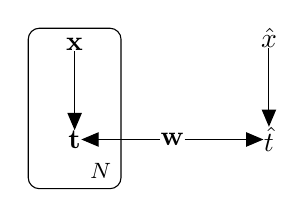
\begin{tikzpicture}

      % Define nodes
	  \node[const]                             (x) {$\quad\mathbf{x}\quad$};   % make it wider for enough plate width
	  \node[const, below=of x]                 (t) {$\mathbf{t}$};
	  \node[const, right=of t]                 (w) {$\mathbf{w}$};
    \node[const, right=of w]                 (t-hat) {$\hat{t}$};
    \node[const, above=of t-hat]             (x-hat) {$\hat{x}$};

	  % Connect the nodes
	  \edge {x,w} {t} ;
	  \edge {x-hat,w} {t-hat} ;

	  % Plates
	  \plate {xt} {(x)(t)} {$N$} ;

	\end{tikzpicture}
  & \quad

  % 2nd
  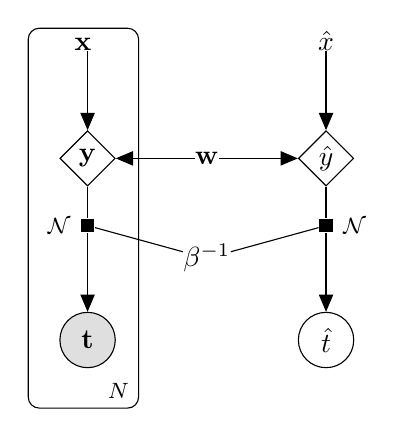
\begin{tikzpicture}

    % Define nodes
    \node[const]                             (x) {$\quad\mathbf{x}\quad\ $};
    \node[det, below=of x]                   (y) {$\mathbf{y}$};
    \node[const, right=of y]                 (w) {$\mathbf{w}$};
    \node[const, below=of w]                 (beta) {$\beta^{-1}$};
    \node[det, right=of w]                   (y-hat) {$\hat{y}$};
    \node[const, above=of y-hat]             (x-hat) {$\hat{x}$};
    \factor[below=of y]{t-f}{left:$\mathcal{N}$}{}{};
    \factor[below=of y-hat]{t-hat-f}{right:$\mathcal{N}$}{}{};
    \node[obs, below=of t-f]                 (t) {$\mathbf{t}$};
    \node[latent, below=of t-hat-f]          (t-hat) {$\hat{t}$};

    % Connect the nodes
    \edge {x,w} {y} ;
    \edge {x-hat,w} {y-hat} ;
    \factoredge{y,beta}{t-f}{t}
    \factoredge{y-hat,beta}{t-hat-f}{t-hat}

    % Plates
    \plate {xt} {(x)(y)(t-f)(t-f-caption)(t)(y.east)} {$N$} ;

  \end{tikzpicture}

  & \quad

  % 3rd
  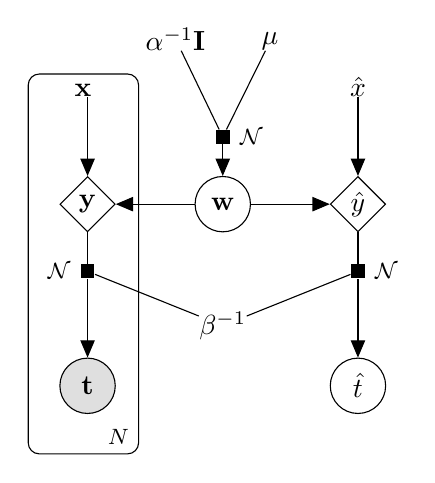
\begin{tikzpicture}

    % Define nodes
    \node[const]                             (x) {$\quad\mathbf{x}\quad\ $};
    \node[det, below=of x]                   (y) {$\mathbf{y}$};
    \node[latent, right=of y]                (w) {$\mathbf{w}$};
    \node[const, below=of w]                 (beta) {$\beta^{-1}$};
    \node[det, right=of w]                   (y-hat) {$\hat{y}$};
    \node[const, above=of y-hat]             (x-hat) {$\hat{x}$};
    \factor[above=of w]{w-f}{right:$\mathcal{N}$}{}{};
    \node[const, above=of w-f, xshift=.6cm]  (mu) {$\mathbf{\mu}$};
    \node[const, above=of w-f, xshift=-.6cm]   (alpha) {$\mathbf{\alpha}^{-1}\mathbf{I}$};
    \factor[below=of y]{t-f}{left:$\mathcal{N}$}{}{};
    \factor[below=of y-hat]{hat-f}{right:$\mathcal{N}$}{}{};
    \node[obs, below=of t-f]                   (t) {$\mathbf{t}$};
    \node[latent, below=of hat-f]                 (t-hat) {$\hat{t}$};

    % Connect the nodes
    \edge {x,w} {y} ;
    \edge {x-hat,w} {y-hat} ;
    \factoredge{mu, alpha}{w-f}{w}
    \factoredge{y,beta}{t-f}{t}
    \factoredge{y-hat,beta}{hat-f}{t-hat}

    % Plates
    \plate {xt} {(x)(y)(t-f)(t-f-caption)(t)(y.east)} {$N$} ;

  \end{tikzpicture}
  \\
  \\(a). LSE & (b) MLE & (c) MAP \& Full Bayesian

  \end{tabular}
  \end{center}
  \caption{Polynomial curve fitting models in PRML: (a) Least Square Estimation in \$1.1; (b) Maximum Likelyhood Estimation (point estimation) in \$2.5; (c) MAximum Posterior estimation (point estimation) in \$2.5 and full bayesian approach in \$2.6}
\end{figure}

\end{document}
